\chapter{Resultados}

En este capítulo se presentan los resultados obtenidos durante la ejecución de la aplicación desarrollada. Se analiza el comportamiento de cada uno de los componentes implementados y se verifica el cumplimiento de los objetivos propuestos al inicio del proyecto.

\section{Escena final}

La Figura \ref{fig:escena_general} presenta el resultado final de la simulación.

Puede observarse la integración de todos los componentes desarrollados durante el proyecto:

\begin{itemize}

\item Sistema de partículas para representar la lluvia.

\item Terreno texturizado.

\item Árboles implementados mediante billboards.

\item Cámara libre con desplazamiento en el plano XZ.

\item Sonido ambiental de lluvia.

\item Interfaz gráfica para modificar parámetros en tiempo real.

\item Efectos meteorológicos de relámpagos.

\end{itemize}

\begin{figure}[H]
\centering
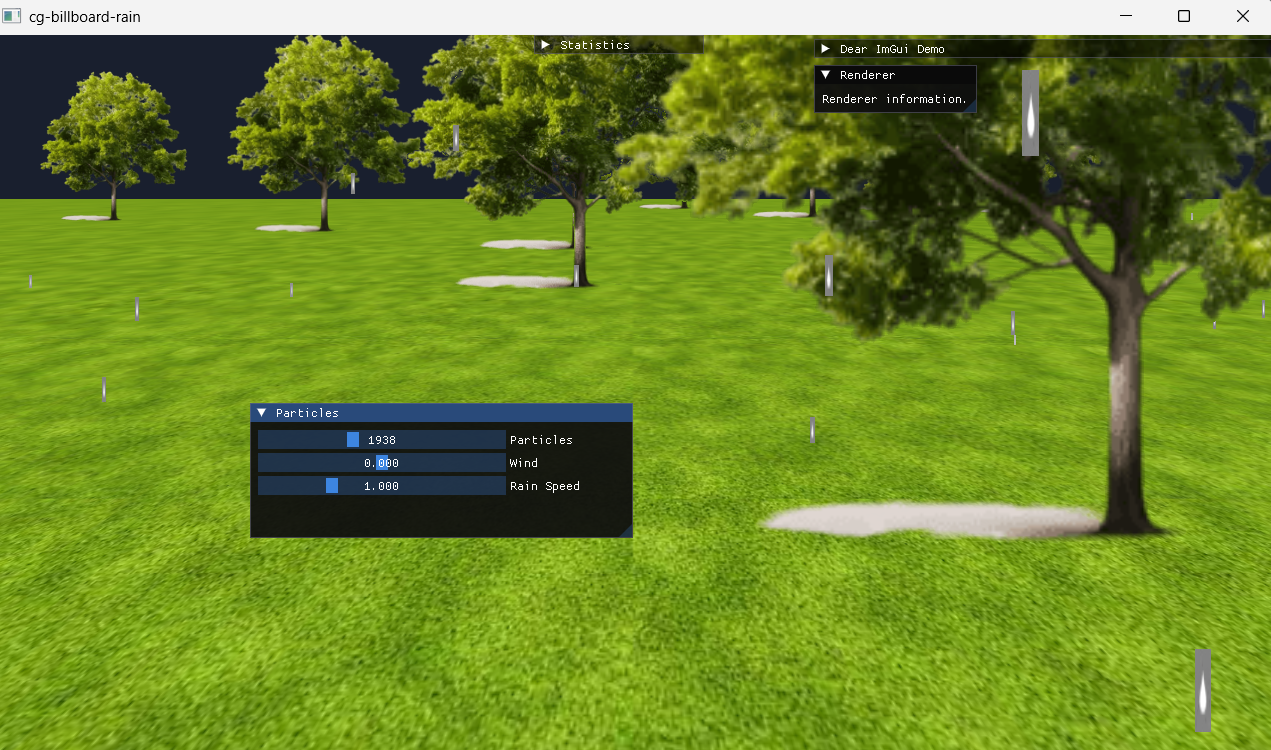
\includegraphics[width=0.9\textwidth]{images/demo.png}
\caption{Resultado general de la simulación.}
\label{fig:escena_general}
\end{figure}

\section{Sistema de partículas}

El sistema de partículas logró representar una lluvia continua utilizando miles de partículas renderizadas simultáneamente.

Cada partícula posee un comportamiento independiente, incluyendo posición, velocidad y reinicio automático al abandonar la zona visible.

Gracias al uso de billboards, todas las partículas permanecen orientadas hacia la cámara, generando una representación visual consistente desde cualquier punto de observación.

La reconstrucción dinámica del sistema permite modificar la cantidad de partículas desde la interfaz gráfica sin necesidad de reiniciar la aplicación.

\section{Sistema de árboles}

Los árboles fueron implementados utilizando billboards de gran tamaño con texturas PNG que incluyen canal alfa.

Cada árbol mantiene siempre su orientación hacia la cámara, simulando modelos tridimensionales con un costo computacional muy reducido.

El algoritmo implementado evita el solapamiento entre árboles mediante una distancia mínima de separación.

Además, cuando un árbol abandona el radio de simulación alrededor del usuario, éste es reposicionado automáticamente delante de la cámara, manteniendo constante la densidad del bosque.

\section{Terreno}

El terreno consiste en un plano texturizado que sigue continuamente la posición horizontal de la cámara.

Este enfoque evita la necesidad de generar un escenario extremadamente grande, reduciendo considerablemente la cantidad de geometría procesada.

Desde la perspectiva del usuario, el terreno aparenta extenderse indefinidamente en todas las direcciones, produciendo una sensación de desplazamiento continuo.

\section{Interfaz gráfica}

La interfaz desarrollada con Dear ImGui permitió modificar diversos parámetros de la simulación durante su ejecución.

Entre los controles disponibles se encuentran:

\begin{itemize}

\item Cantidad de partículas.

\item Intensidad del viento.

\item Velocidad de caída de la lluvia.

\item Información del rendimiento.

\item Posición de la cámara.

\end{itemize}

Las modificaciones realizadas desde la interfaz se reflejan inmediatamente sobre la simulación, permitiendo experimentar distintos escenarios climáticos en tiempo real.

\section{Sistema de audio}

La incorporación de sonido ambiental incrementó significativamente la sensación de inmersión.

El audio de lluvia se reproduce continuamente durante la ejecución del programa.

Su intensidad y velocidad de reproducción cambian automáticamente de acuerdo con la cantidad de partículas presentes en la escena.

De esta manera, una lluvia más intensa produce también una percepción auditiva más fuerte y dinámica.

\section{Sistema meteorológico}

El sistema meteorológico implementado añade relámpagos aleatorios durante la simulación.

Cada relámpago incrementa temporalmente la iluminación del fondo mediante una modificación dinámica del color utilizado por el renderizador.

Posteriormente la intensidad disminuye progresivamente hasta recuperar el estado normal de la escena.

Este efecto visual contribuye a representar una tormenta de manera más realista sin incrementar significativamente el costo computacional.

\section{Evaluación del rendimiento}

Durante las pruebas realizadas se observó un comportamiento estable incluso utilizando varios miles de partículas simultáneamente.

La utilización de billboards para representar tanto la lluvia como los árboles permitió mantener un bajo consumo de memoria y una carga reducida sobre la GPU.

La interfaz gráfica mostró continuamente la cantidad de cuadros por segundo (FPS), permitiendo monitorear el rendimiento de la aplicación mientras se modificaban los parámetros de la simulación.

En equipos con aceleración gráfica compatible con OpenGL 3.3, la simulación mantiene una ejecución fluida para configuraciones de hasta 5000 partículas de lluvia.

\section{Discusión}

Los resultados obtenidos demuestran que es posible construir una simulación visualmente atractiva utilizando técnicas relativamente simples como billboards, sistemas de partículas y renderizado mediante OpenGL.

La arquitectura modular implementada facilitó el desarrollo incremental del proyecto y permitió incorporar nuevas funcionalidades sin modificar significativamente los componentes existentes.

Asimismo, la integración del sistema de audio y los efectos meteorológicos incrementó el nivel de realismo alcanzado por la simulación, ofreciendo una experiencia más inmersiva para el usuario.